\documentclass[a4paper, 11pt]{article}
\usepackage[text={17cm, 24cm}]{geometry}
\usepackage[czech]{babel}
\usepackage[T1]{fontenc}
\usepackage{hyperref}
\usepackage{lmodern}
\usepackage{sourcecodepro}
\usepackage{minted}
\usepackage{graphicx}
\usepackage{hyperref}
\usepackage{booktabs}
\usepackage{longtable}

\setminted{ 
    tabsize=4, 
    fontsize=\footnotesize, 
    encoding=utf8,
    escapeinside=||
}

\setlength{\LTcapwidth}{\textwidth}

\title{\huge KRY -- protokol k~prvnímu projektu}
\author{Ondřej Koumar, xkouma02 (241550)}
\date{\today}

\begin{document}

\maketitle

\section{Postup řešení}\label{kap:postup_reseni}

Jako první jsem potřeboval zjistit, jakou kódovou knihu použít pro dešifrování původních zpráv, které obsahovaly pouze znaky ve formátu \texttt{\textbackslash xDD}, kde \texttt{D} je zástupný symbol pro libolnou číslici z~množiny $\{0, \ldots, 9\}$.
Na obrázku \emph{spaceship.jpg} jsem si samozřejmě všimnul velkého nápisu \emph{VUT ID MOD 10}.
Naivně jsem si myslel, že jsem vyhrál a~začal jsem dešifrovat, k~čemuž jsem si napsal malý script v~Pythonu.
Disclaimer: asi to není nejčistší kód, ale svoji práci to dělá.

\label{code:desifrovaci_skript}
\begin{minted}[linenos=false]{python3}
    encryption = { # tento slovnik byl menen dle pouzivane kodove knihy
        "x08": "a",
        "x36": "b",
        "x54": "c",
        |\phantom{xxxxx}\vdots|
        "x25": "zz"
    }

    i = 0
    all_messages = ""
    with open("../cipher.txt") as f:
        for line in f:
            decrypted_message = ""
            for encrypted_char in line.replace(',', '').strip().split():
                decrypted_char = encryption[encrypted_char]
                decrypted_message += decrypted_char
            print(f"ZP{i}: {decrypted_message}")
            all_messages += decrypted_message + "\n"
            i += 1
            decrypted_message = ""

    list_of_messages = []
    for message in all_messages.split('\n'):
        list_of_messages.append(list(message))
    
    messages_csv_format = ""
    for message in list_of_messages:
        for char in message:
            messages_csv_format += char + ';'
        messages_csv_format += '\n'
    
    with open("output.csv", 'w') as f:
        f.write(messages_csv_format)
\end{minted}

Po dešifrování zpráv kódovou knihou, kterou jsem vybral pomocí modulování mého VUT ID, jsem nedošel vůbec nikam.
Dlouho mi trvalo, než jsem se přemluvil, abych přestal s~dešifrováním zprá\-vy a~znovu se podíval, jestli jsem si vůbec vybral správnou kódovou knihu.
Tento první pokus jsem prováděl metodou tužka-papír a~snažil jsem se najít souvislosti mezi mezi písmenky -- použil jsem frekvenční analýzu a~další metody, ze kterých jsem nic nezjistil.
Bohužel už přesně nevím, co všechno jsem zkoušel, začínal jsem zhruba dva týdny před psaním této zprávy a~nepamatuji si všechny své experimenty.
Navíc, z~frustrace jsem všechny papíry popsané neúspěšným prvním pokusem vyhodil.

Začal jsem se na situaci dívat \emph{jinak}.
Přesněji, na obrázek \emph{spaceship.jpg} jsem se začal dívat jinak.
Bylo mi jasné, že v~něm musí být schované něco, co bych mohl využít.
Po pár minutách jsem usoudil, že samotné hledání detailů na obrázku nemá smysl a~zkusil jsem se podívat do vlastností samotného souboru.
Co jsem našel je ukázáno na Obrázku \ref{fig:prirazeni_kodovych_knih}.

\begin{figure}[t]
    \centering
    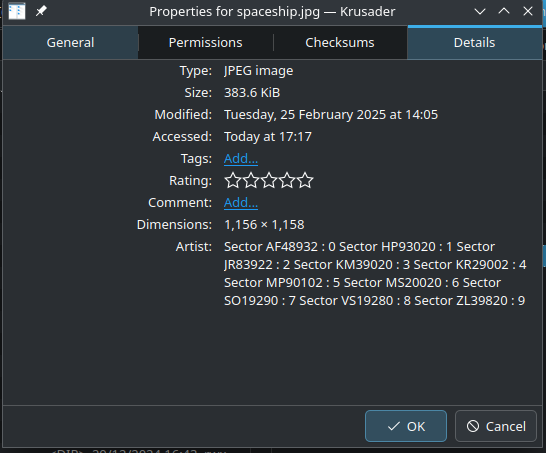
\includegraphics[width=0.7\textwidth]{img/hidden_codebook_sectors.png}
    \caption{Schovaná přiřazení různých kódových knih podle zbytku VUT ID po dělení 10.}
    \label{fig:prirazeni_kodovych_knih}
\end{figure}

Bylo mi tedy jasné, že musím opravdu svoje VUT ID vydělit 10, ale poté vybrat kódovou knihu, na základě zbytku po dělení, z~rozdělení definovaného v~sekci \emph{Artist}.
Protože zbytek po dělení mého VUT ID 10 je 0, vybral jsem kódovou knihu \emph{Sector AF48932}.
Zprávy po dešifrování kódovou knihou jsou v~Tabulce \ref{tab:desifrovane_zpravy_codebook}.

\begin{table}[h]
    \centering
    \begin{tabular}{l l}
        \toprule 
        \textbf{Číslo zprávy} & \textbf{Dešifrovaná zpráva} \\
        \midrule
        ZP0 & rmxesxzoxvaotyhntaaolsntvienaiernovsceolaviptemppbztnnoueelr \\
        ZP1 & nixctxisxajxattirecovziiaeieaemdtnpltackikobeunlaaxtaxszxnta \\
        ZP2 & vxapmxrixeakkimurhopixruave2nv0edmanrtlcttyiiksemnlnmeaaciye \\
        ZP3 & dlxyyxbvxnexsyacaeesdvvsnecdckykehdkoknynpnaareaspvavltoevao \\
        ZP4 & unvosxtaaieaeulaedknockierlattniompfollvkptsapeizninjreuprer \\
        ZP5 & vexhdxaaxorxoanmnlrvaflyckzanneaeaiofntjaranoloehietyaotdebp \\
        ZP6 & eznimxvainaleirranptendettolcreibikaaanjosstankaspaeditebert \\
        ZP7 & ikxiuxnnxlcxrhyratolupitznctpaiinavobcoatmriroofnccuaxohenaa \\
        \bottomrule 
    \end{tabular}
    \caption{Zprávy po prolomení substituční šifry pomocí kódové knihy.}
    \label{tab:desifrovane_zpravy_codebook}  
\end{table}

Tímto momentem jsem se dostal do fáze lámání zašifrovaného textu.
Druhá část projektu šla mnohem rychleji než první.
Když se podíváte na \hyperref[code:desifrovaci_skript]{skript}, který jsem si pro potřeby řešení tohoto projektu vytvořil, zjistíte, že všechny dešifrované zprávy ukládám bez jakýchkoliv dalších informací do \emph{.csv} souboru.
Tento \emph{.csv} soubor jsem si otevřel v~tabulkovém procesoru s~myšlenkou, že se mi v~něm bude lépe pracovat než na papíře.
Trvalo mi jen pár minut zjistit, že to byl lepší nápad, než jsem původně očekával.
To díky možnosti hýbat s~celými sloupci v~tabulkových procesorech (možná je to čtenáři dlouho známý fakt, ale pro mě to byla úplná novinka), navíc šifra byla postavená tak, že se dala vyřešit přeskupováním sloupců a~postupným doplňováním slov tak, aby dávaly smysl.
Jak to v~tabulkovém procesoru vypadalo je ukázáno na Obrázku \ref{fig:work_in_libreoffice}.

\begin{figure}[ht]
    \centering
    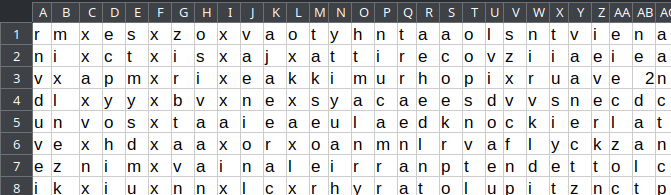
\includegraphics[width=0.7\textwidth]{img/work_in_libreoffice.png}
    \caption{Náhled na práci se zašifrovanými zprávami v~tabulkovém procesoru. Část šifer je uříznuta, aby se obrázek pohodlně vlezl na šířku stránky a~zároveň byl čitelný.}
    \label{fig:work_in_libreoffice}
\end{figure}

Když se podíváme na zprávu \emph{ZP2}, najdeme v~ní, jako jediné, čísla.
Jsou to stejná čísla, která mám v~xloginu, proto jsem svoji práci začal sestavením xloginu tak, aby písmena v~jiných řádcích také dávala smysl, což se po pár pokusech podařilo. 
Prozatím jsem jej ponechal na začátku řádku s~tím, že v~případě potřeby jej přehodím jinam, nicméně nakonec tam zůstal, před něj už žádný sloupec nešel.

Postupně jsem zprava skládal sloupce, dokud jsem se na chvíli nezasekl, protože jsem měl vícero možností, které by dávaly smysl.
Abych zredukoval počet těchto možností, začal jsem skládat od konce.
Všiml jsem si, že v~každém řádku je několik písmenek \texttt{x}, v~jednom sloupci byly dokonce ve všech řádcích.
Napadlo mě, že sloupec s~\texttt{x} na konci by mohl značit konec řádku nebo něco podobného a~zkusil jsem jej dát na konec.
Poté jsem si všiml sloupců, ve kterých bylo písmenek \texttt{x} dost, i~když ne všechny.
Dospěl jsem k~tomu, že každý řádek bude jinak dlouhý a~\texttt{x} na konci budou výplní, aby všechny zprávy byly stejně dlouhé.
Po pár minutách zkoušení a~přehazování jsem se dostal do fáze, kdy písmenka na koncích řádků začala vypadat jako části slov.
V~tu chvíli už skládání šlo opět rychle.
Tímto způsobem jsem pokračoval, dokud jsem celou šifru neměl poskládanou tak, aby dávala smysl.
Pokud v~ní byl nějaký sofistikovanější systém, který se dal najít, já ho nenašel.

\subsection{Shrnutí}

Pří řešení projektu jsem dešifroval původní zprávy ve dvou krocích.
V~prvním kroku jsem překonal substituční šifru, která byla realizována kódovou knihou.
Druhý krok byl lámání transpoziční šifry.
Během řešení jsem nepřišel na přesný systém, kterým jsou sloupce přeházeny, projekt jsem vyřešil pomocí posouvání sloupců doleva a~doprava, dokud písmenka začala dávat smysl a~postupným přidáváním dalších sloupců ke zprávě zprava.
Paralelně jsem skládal zprávu od konce, protože jsem si všiml spousty písmenek \texttt{x}, pomocí kterých se mi povedlo dát dohromady části slov na koncích řádků.
Mezi těmito dvěma částmi jsem přeskakoval, když jsem měl vícero možností, jak pokračovat.

\section{Dešifrované zprávy v plaintextové podobě}

\begin{longtable}{ll}
    \toprule
    \textbf{Číslo zprávy} & \textbf{Dešifrovaná zpráva po prolomení transpoziční šifry} \\ 
    \midrule
    \endhead
    ZP0 & \texttt{stanovenecilepotvrzenyotviramepalbunamosthlasenipotvrzenoxxx} \\ 
    ZP1 & \texttt{zacinameutoknastanicitorpedanabitazajistitvelitelcekaxxxxxxx} \\
    ZP2 & \texttt{xkouma02krycimanevrpripravenstitynamaximumihnedvelitelcekaxx} \\
    ZP3 & \texttt{vsechnydronyvstandbyvysadekcekanapovelvysadekcekanapovelxxxx} \\
    ZP4 & \texttt{cekamenapotvrzeniutokunepritelskenujenasilodflotilapripravax} \\
    ZP5 & \texttt{formacealfajehotovahlavnikanonnabityreadynalozenetorpedaxxxx} \\
    ZP6 & \texttt{nepritelnasjesteneviditaktickatorpedazamerenaobranastabilnix} \\
    ZP7 & \texttt{prorazitobrannouliniihlavnipocitachacknutyutocnaformacexxxxx} \\
    \bottomrule
    \addlinespace[8.5pt]
    \caption{Dešifrované zprávy po prolomení substituční šifry (kódová kniha) a~transpoziční šifry.}
\end{longtable}


\end{document}